\chapter{Generalization of the Attack}
\label{chap:Generalization}

So far, our attack is only based on one single environment. The attacker trains and tests his attack on the same pair of devices with data collected at roughly the same point in time. In this chapter, we explore a generic context, where an attacker test his attack on other devices and with time delays.

\section{Transferability}
We want to show that an attacker learning on a particular smartwatch-phone pair can also detect applications on another smartwatch-phone. This would benefit greatly an attacker, since one single pair of devices would allow him to target many possible others. 
\\

We took the Huawei-Pixel and Fossil-Nexus dataset, from Chapter~\ref{chap:analysis_and_results}, learned the model on one pair, test on the other and vice versa. To allow a fair comparison, we selected a subset of 35 overlapping applications and performed equalization such that the two pairs have the same amount of samples per class. We used all the dataset of one pair for training and tested on all the dataset of the other pair. We achieve \textbf{80.3\% (+/- 0.7\%)} accuracy when training on Huawei and testing on the Fossil and \textbf{85.5\% (+/- 1.3\%)} vice versa. We note that training on Fossil leads to lower accuracy. This is explainable because the overall accuracy when only Fossil is tested is lower. Thus the Fossil dataset is noisier and more difficult to predict. We show the Confusion Matrix in Fig.~\ref{fig:cm transferability}. 
\\

\begin{figure}[h]
\centering
\begin{subfigure}{.5\textwidth}
  \centering
  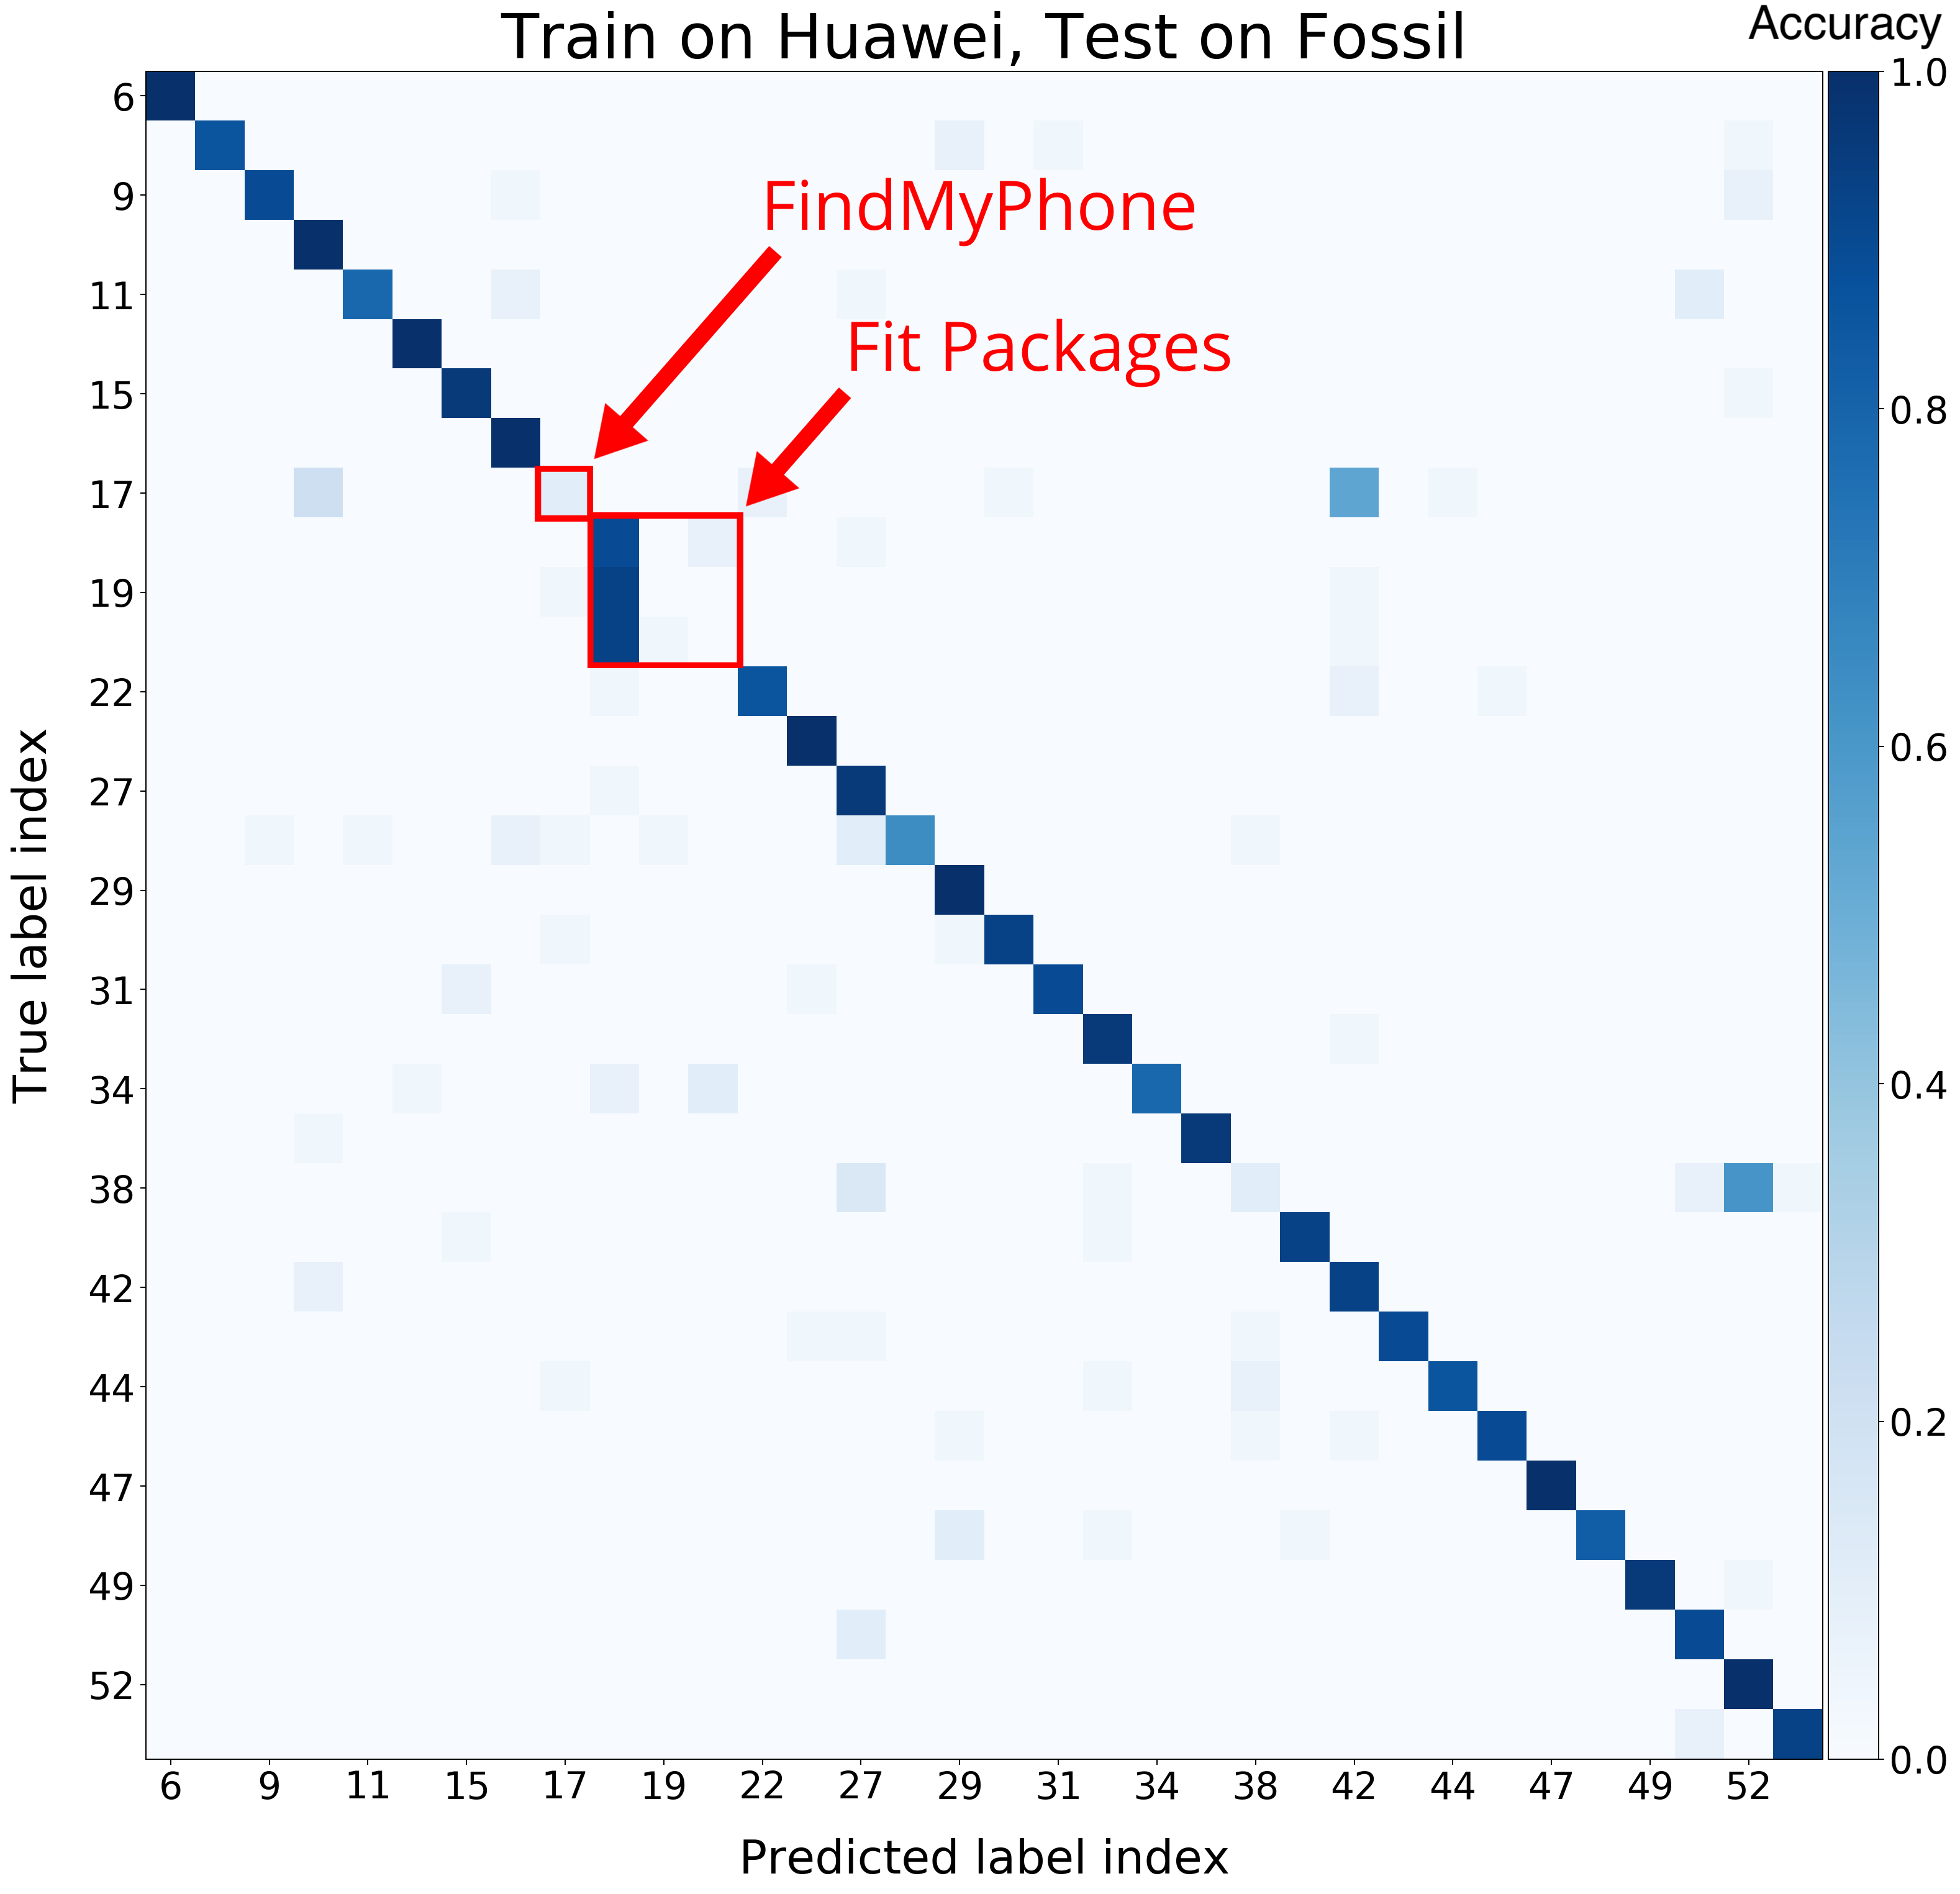
\includegraphics[width=1\textwidth]{figures/cm/Confusion_matrix_train_with_Huawei_test_with_Fossil_annoted.png}
\end{subfigure}%
\begin{subfigure}{.5\textwidth}
  \centering
  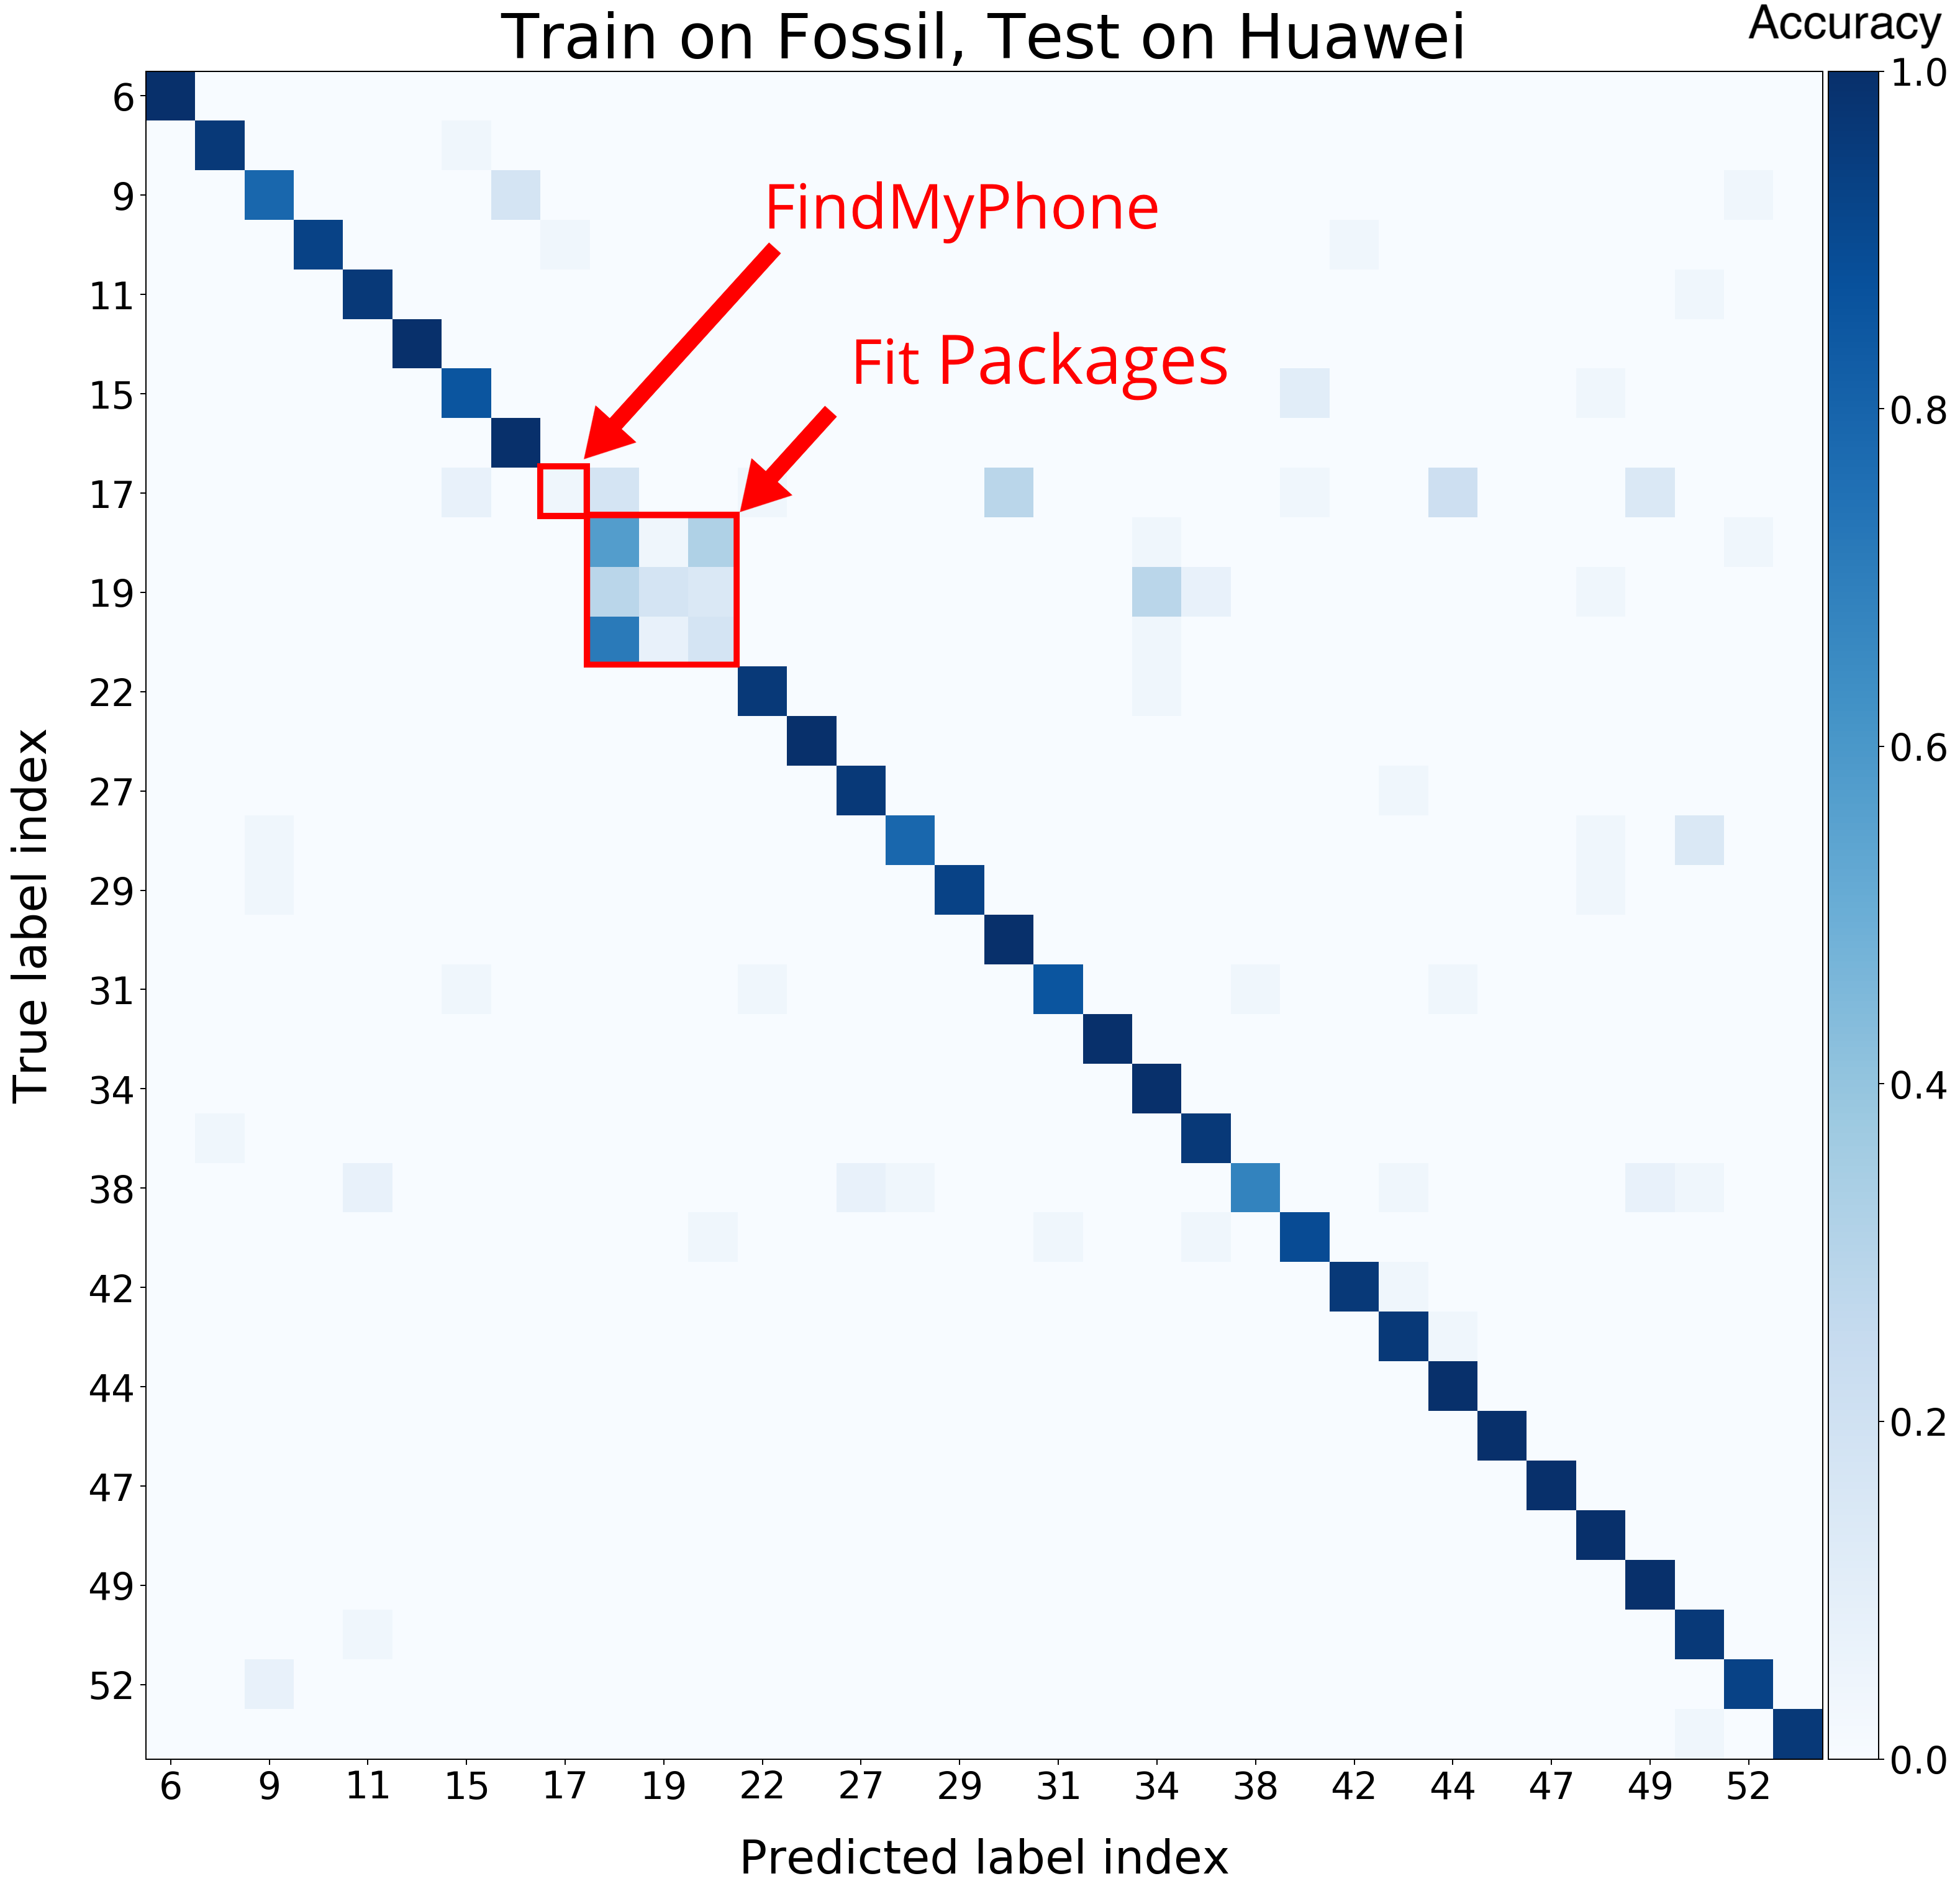
\includegraphics[width=1\textwidth]{figures/cm/Confusion_matrix_train_with_Fossil_test_with_Huawei_annoted.png}
\end{subfigure}
\caption{\textbf{Left:} Attacker learn on Huawei, test on Fossil \textbf{Right:} Attacker learn on Fossil, test on Huawei}
\label{fig:cm transferability}
\end{figure}
\newpage
We notice that only few applications lower the accuracy. FindMyPhone, for instance does not achieve more than 15\% accuracy score in both experiments. FindMyPhone\footnote{\textbf{FindMyPhone} is an application on smartwatches that rings the phone when triggered.} is an application that relies highly on the phone and its operating system, thus explaining why we do not expect to achieve more accuracy on this application. Moreover, we also see that apps coming from the Fit packages also do not achieve good results. We knew already that these apps are noisier since they are from the same package. By grouping the Fit packages into one entity, we found an accuracy of \textbf{86.1\% (+/- 0.7\%)} and \textbf{90.1\% (+/- 1.1\%)} for Huawei train and Fossil test and vice versa. Overall, the attack transfers very well apart from few specific applications.

\section{Evaluation over Time}
\label{sec:eval over time}
One could argue that the model we develop is too specific to one particular environment. i.e. the training set of the attacker is acquired in the same condition than the testing set. Network conditions might vary, the content of applications might change over time (such as maps or news applications), and application updates might also impact the traffic\footnote{Unfortunately, we did not track software updates of application and OS updates. However, updates happen more often than we expected. We recorded that in six days (from April 22nd 2020 to April 28th 2020), 11 software updates from different packages have been updated in the background.}. In 2014, Juarez et al. formulated the same critic towards WF, using previous work, they show that after 5 days accuracy dropped from around 80\% to less than 50\%\cite{juarez2014critical}. Taylor et, al. also formulated critics along these lines for MAF~\cite{taylor2017robust}. Therefore, even though an attacker can update his dataset to keep fresh data, we ask ourselves how accuracy will decrease with ageing and how frequent should an attacker updates its dataset.
\\

We collected, over 33 days, 11 set of captures at 4 days interval except for the first two days where we also performed captures. We initially took a subset of 33 applications and generated 10 captures per application on a "capture" day. However, at day 20, we realised that an update arose on the applications belonging to the Fit package, making them not transferring data anymore. So we put these apps aside and continued with only fingerprintable applications. The blue line in Fig.~\ref{fig:accuracy over time} shows the accuracy over time when trained with the dataset at day 0 and test with the dataset at day n. The red dotes are the accuracy when the training and testing dataset are from the same day. 

\begin{figure}[H]
 \centering
 \includegraphics[width=0.7\textwidth]{figures/plots/Accuracy_over_time_c08to1_train_only0_bis2.png}
 \caption{Accuracy over time }
 \label{fig:accuracy over time}
\end{figure}

\newpage

First, we note that the accuracy when we train and test on the same day have a slight variations (+/- 3\%) across days this confirmed our experiment on dataset size (see Sec.~\ref{data_set_size_per_class}). As expected there is a small accuracy decrease of 3.7\% on average between the blue line and the red dotes showing that, over time, the attack is weakened. Now, the question is how is this noise distributed over the classes. To see that, we averaged the accuracy loss over all days separated by class (See Fig.~\ref{fig:acc gain overtime}). We distinguish two things from this plot. First, except few apps that have small positive accuracy gain (or no gain), most apps are loosing accuracy over time. Moreover, one package has almost 50\% accuracy loss: DCLMRadio, a christian radio broadcast application. We explain this by observing the following: this application directly fetches a large amount of data from a remote sever at startup, and we suspect that errors occur frequently on their server which changes radically the communication scheme for specific days. In addition, two other apps show significant losses of more than 10\%: Google Map and Outlook.
\\
\begin{figure}[ht]
 \centering
 \includegraphics[width=0.70\textwidth]{figures/plots/accuracy_gain_per_class_when_mix_trained_j=all.png}
 \caption{Accuracy gain per class averaged over all days.}
  \label{fig:acc gain overtime}
\end{figure}

To reduce the accuracy drop caused by ageing, we trained the model on the first three days of the experiment instead of the first day alone, but with keeping the same dataset size to ensure fair comparison. We reproduce the graph from Fig.~\ref{fig:accuracy over time} and \ref{fig:acc gain overtime} in Fig.~\ref{fig:learning extension over time}.


\begin{figure}[h]
\centering
\begin{subfigure}{.5\textwidth}
  \centering
  \includegraphics[width=1\textwidth]{figures/plots/Accuracy_over_time_c08to1_train_only0_bis2_mix.png}
\end{subfigure}%
\begin{subfigure}{.5\textwidth}
  \centering
  \includegraphics[width=1.05\textwidth]{figures/plots/accuracy_gain_per_class_when_mix_trained_j=all_mix2.png}
\end{subfigure}
\caption{\textbf{Left:} Accuracy over time when trained with day 0, 1, and 2 \textbf{Right:}Accuracy gain averaged over time by class}
\label{fig:learning extension over time}
\end{figure}

\newpage

By doing this learning adjustment, we lower the average accuracy drop between current and delayed training from 3.7\% to 0.37\%. We can see now that the blue curve follows the red dotes. Interestingly, we could even achieve better results at day 20, which shows that the model can also learn better features when the training environment is changed. Indeed, if we look at the right part of Fig.~\ref{fig:learning extension over time}, we see that four applications achieved better results on average. Amongst them, ChinaDaily, a news app where content is updated frequently. Also, we could significantly lower the loss of DCLMRadio application (leftmost bar) by about a half. 
\\

To answer the question how frequent an attacker should refresh its dataset, we can say that after 32 days, 3.7\% is not a huge loss. However, some applications might suffer much more from ageing than others, and therefore an attacker wanting to be consistent over all its targeted actions might want to perform more frequent updates. Moreover, to counterbalance the effect of ageing, and to perform less updates, an attacker might want to train his model over few days.

